% Modified based on Xiaoming Sun's template

% Modified based on Xiaoming Sun's template

\documentclass{article}
\usepackage{amsmath,amsfonts,amsthm,amssymb}
\usepackage{indentfirst}
\usepackage{setspace}
\usepackage{fancyhdr}
\usepackage{lastpage}
\usepackage{extramarks}
\usepackage{chngpage}
\usepackage{soul,color}
\usepackage{graphicx,float,wrapfig}
\usepackage{ifpdf}
%\usepackage{CJKspace}
\usepackage{verbatim}
%\usepackage{ctex}
\usepackage{algorithm}
\usepackage{algorithmicx}
\usepackage{algpseudocode}
\usepackage{url}

%\usepackage{natbib}

\usepackage[colorlinks, citecolor=blue]{hyperref}


% In case you need to adjust margins:
% \topmargin=-0.45in      %
% \evensidemargin=0in     %
% \oddsidemargin=0in      %
% \textwidth=6.5in        %
% \textheight=9.0in       %
% \headsep=0.25in         %

% Setup the header and footer
% \pagestyle{fancy}                                                       %
% \chead{\Title}  %
% \rhead{\firstxmark}                                                     %
% \lfoot{\lastxmark}                                                      %
% \cfoot{}                                                                %
% \rfoot{Page\ \thepage\ of\ \protect\pageref{LastPage}}                          %
% \renewcommand\headrulewidth{0.4pt}                                      %
% \renewcommand\footrulewidth{0.4pt}                                      %

% �����Զ���һЩ����
\newcommand{\Answer}{\ \\\textbf{Answer:} }
\newcommand{\Acknowledgement}[1]{\ \\{\bf Acknowledgement:} #1}
\newcommand{\Reference}[1]{\ \\{\bf Reference:} #1}
\newtheorem{theorem}{Theorem}

\newcommand\numberthis{\addtocounter{equation}{1}\tag{\theequation}}


    %%%%%%%%%%%%%%%%%%%%%%%%%%%%%%%%%%%%%%%%%%%%%%%%%%%%%%%%%%%%%


    %%%%%%%%%%%%%%%%%%%%%%%%%%%%%%%%%%%%%%%%%%%%%%%%%%%%%%%%%%%%%
    % ���ⲿ��
    \title{\textmd{\bf Artificial Intelligence Project -- Final Report}}
    \date{}
    \author{Yiheng Lin, Zhihao Jiang}
    %%%%%%%%%%%%%%%%%%%%%%%%%%%%%%%%%%%%%%%%%%%%%%%%%%%%%%%%%%%%%

    \begin{document}
    \begin{spacing}{1.1}
    \maketitle %\thispagestyle{empty}

    %%%%%%%%%%%%%%%%%%%%%%%%%%%%%%%%%%%%%%%%%%%%%%%%%%%%%%%%%%%%%
    % Begin edit from here
    \section{Introduction and Background}
    The foundation of h-DQN should be deep Q-learning method proposed by the authors of \cite{AI-15}. They proposed two important methods to fix the instability when applying deep learning to reinforcement learning, which is memory replay and fixing the parameters of the target network. Their works make it possible to apply the deep Q-learning to solve problems like playing simple games. But the limitation that hinders deep Q-learning to be applied in the real world is that the rewards are often too sparse for the agent to learn good policies efficiently.

    The intuition of h-DQN (Hierarchy Deep Q-Learning) may come from the thought that a big goal can be divided into a sequence of small goals, which are much easier to reach for the agent than the big goal. By reaching a small goal at a time, the agent may be able to handle the situations in which rewards are sparse. So the authors of \cite{AI-16} proposed a structure as following: a meta-controller (the higher hierarchy) is responsible for choosing a goal for the controller (the lower hierarchy) given the sequence of steps and states the controller experiences and the extrinsic reward they get during the process of trying to reach the subgoal; a controller, who tries to reach the goals set by the meta-controller, takes actual actions in the environment and receiving the intrinsic reward designed based on the goal.

    Despite tackling the efficiency problem when rewards are sparse, another two advantages of h-DQN are: it can reveal a hidden state that is crucial for deciding the final reward; it can also encourage the agent to explore unknown states more actively. To make it clear, consider the following game proposed in \cite{AI-16}:

    \subsection{Experiment Game Setting}
    The state set is $S = \{1, 2, \cdots, 6\}$ and the action set is $A = \{1, 2\}$. The agent starts at state 2 and state 1 is the terminal state. At state i, if the agent takes action 1, it will go to state $i-1$ with probability 1; if the agent takes action 2, it will go to state $i+1$ with probability 0.5;otherwise, it will go to state $i-1$. The reward is received at state 1: if the agent has been to state 6, it will receive reward 1; otherwise, it will receive a reward $0.01$.

    \begin{center}
        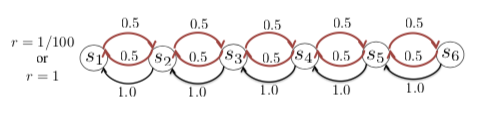
\includegraphics[width = 0.5\textwidth]{game.png}
    \end{center}

    During the presentation, our mentor points out that this is not an MDP (Markov Decision Process) since the reward depends on the whole history rather than the current state and action. But actually this implies a common case we meet in the real situation, that is, we may fail to add some crucial hidden states that decide the final reward to the state space. As we mentioned in the progress report, by adding an additional dimension to the state space which indicates whether we have already visited state 6, the problem will become much easier. But without this additional state, the problem is almost intractable for traditional Q-learning and DQN which tries to approximate the Q function. However, h-DQN, in which the controller is given both state and goal, intrinsically has more dimensions in new state space than the original state space. This may help h-DQN to perform better than traditional Q-learning in this problem.

    Another important function of subgoals are encouraging exploration. Notice that in our problem's setting, random actions can hardly reach state 6. By setting a remote state as a goal, the agent is pushed to explore that state rather than try aimlessly and give up.

    \subsection{Setting Goal and Intrinsic Reward}
    The authors of \cite{AI-18} proposed a way to set goals and intrinsic rewards. In their method, each goal is set to a specific state and intrinsic reward is the opposite number of the l2-norm of the difference of current state and goal state (i.e. $r(s_t, g_t, a_t, s_{t+1}) = -||s_t + g_t - s_{t+1}||$, here $s_t + g_t$ is the goal observation and $s_{t+1}$ is the current observation). As they mentioned, this method works will in the ant grid game setting and can be easilly generallized to tackle other game settings.

    In our experiment, we use the same method to set goals and intrinsic rewards (that is, approaching the goal incurs higher intrinsic rewards). Although our mentor said after our presentation that the distance between two states cannot be easily found, we think the Lp-norm of the difference between the goal and the current state is at least a good heuristic of the real distance (in action steps). And we find this method can significantly accelerate the training process by encouraging the controller (the lower hierarchy) to achieve the goal and give more accurate feedback to the meta-controller (the higher hierarchy).

    \subsection{Limitations of the previous works}
    We have carefully studied the h-DQN algorithm proposed in \cite{AI-16} and reimplement their method based on \cite{github} to solve the problem we mentioned in subsection 1. A significant weakness of this method is the performance is too volatile and seems very hard to converge. And as we observed, in the actual training process, the learning of meta-controller and controller did not follow the authors' expectation. When the subgoal is set to state 2, the controller (the lower hierarchy) opts to choose action 2 frequently even when it is at state 3, 4, 5 and consequently arrives at state 6 with high probability. This encourages the meta-controller (the higher hierarchy) to set the subgoal to state 2 since the meta-controller will see setting subgoal 2 often results in a good extrinsic reward. The reason may be that the experience provided to the meta-controller is highly unstable during the training. The controller may have learned a suboptimal policy to reach its subgoal, but this suboptimal policy results in a good extrinsic reward, which is favored by the meta-controller. When we see good average rewards, the model may have not converged. And maybe at some time the controller may find a new way to reach its subgoal, then the average reward collapses dramatically, as we see when running experiment.

    To choose goal space, the authors of \cite{AI-16} said we can find (manually or by some digital image processing skill) some things that are very possible to be important for this game. They argued that labeling objects in a given image (for example, find the key, ladders etc. in ATARI game) is an open problem. So we do not consider how to find the goal set when studying h-DQN. And the authors of \cite{AI-18}, claims that letting the goal states as the state space can more easily be generallized. However, this method might only be useful in games that have a very good and thorough abstraction. If the agent can only discover a small part of the whole environment, we cannnot easily apply their method.

    And we find this weakness of generalization when we try to apply the h-DQN method to learn a control policy in the flappy bird game. We first do the experiment using DQN method based on the code on \cite{github2}.
    \begin{center}
        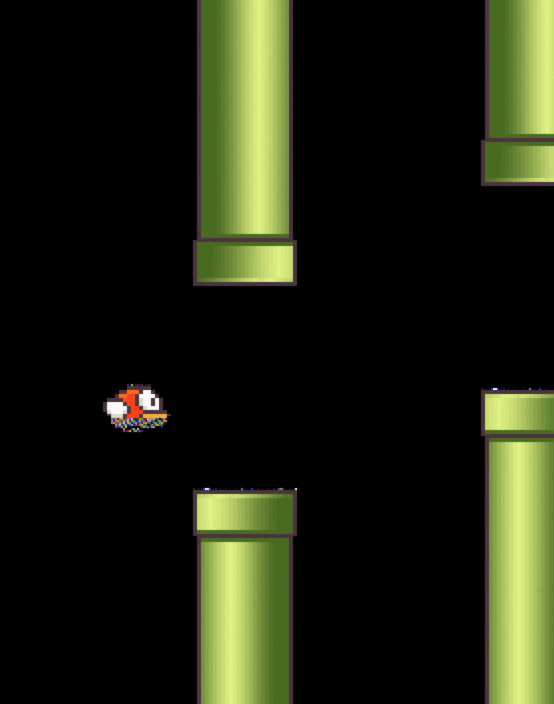
\includegraphics[width = 0.5\textwidth]{Fluppy.png}
    \end{center}
    
    Although we can observe the improvement through time, the agent learns very slow. This may because the (extrinsic) reward is given only when the bird has successfully passed through a door. At many times, although the bird has reached the height that can pass the door or very close to the door, it crashes into the wall due to some small disturb. Then the agent cannot distinguish this case with the totally bad policy like always flying upward because it does not receive any additional reward for getting more closer to the door. If we use the h-DQN method, we can set a goal in the door and give intrinsic to the controller for getting closer to this goal. Then this may speed up the training process. But since the scene is changing and moving forward, we cannot fix a location or a specific image as the goal for controller. Even reading the current height of the bird requires a new neural network and additional training, and requires specific human knowledge of the rules of this flappy bird game.

    \bibliographystyle{plain}
    \bibliography{refx}

    %\Acknowledgement{}

    % End edit to here
    %%%%%%%%%%%%%%%%%%%%%%%%%%%%%%%%%%%%%%%%%%%%%%%%%%%%%%%%%%%%%

    \end{spacing}
    \end{document}

    %%%%%%%%%%%%%%%%%%%%%%%%%%%%%%%%%%%%%%%%%%%%%%%%%%%%%%%%%%%%%

